% !TEX root = rob1.tex
\chapter{Robotermodellierung}
\section{Geometrisches Model}
\mparagraph{Einsatzbereich}
\begin{compactitem}
    \item Graphische Darstellung von Körpern
    \item Ausgangspunkt der Abstandsmessung und Kollisionserkennung
    \item Grundlage zur Berechnung der Bewegungen von Körpern
    \item Grundlage zur Ermittlung der wirkenden Kräfte und Momente.
\end{compactitem}

\mparagraph{Klassifizierung}
\begin{itemize}
    \item \textbf{Raum}: 2D, 2.5D, 3D Modelle
    \item \textbf{Grundprimitive}
    \begin{compactitem}
        \item Kanten- bzw. Drahtmodelle
        \item Flächen- bzw. Oberflächenmodelle
        \item Volumenmodell
    \end{compactitem}
\end{itemize}
\section{Kinematisches Model}
\textbf{Das kinematische Modell eines Roboters beschreibt die Zusammenhänge zwischen
dem Raum der Gelenkwinkel (Roboterkoord, Konfigurationsraum) und dem Raum der
Lage des Endeffektors in Weltkoordinaten (Arbeitsraum, Kartesischer Raum.)}
\section{Direktes kinematisches Problem, Vorwärtskinematik}
\textbf{Bestimmung der Lage des Endeffektors aus den Gelenkwinkelstellungen des Roboter.}

\subsection{Kinematische Kette}
\textbf{Eine kinematische Kette wird von mehreren Körpern gebildet, die durch Gelenke kinematisch
verbunden sind.}

\begin{compactitem}
    \item In jedem Armelement wird ein festes lokales Koordinaten System gelegt (OKS)
    \item Ursprung des Koordinatenszstems liegt im Armgelenk, welches das jeweilige
    Armelement bewegt.
    \item Für jedes Armelement muss eine Transformationsmatrix bestimmt werden, die das jeweilige
    lokale Koordinatensystem in das Bezugskoordinatensystem überführt.
    \item Überführung der lokalen Koordinatensysteme in das Bezugskoordinatensystem durch
    Beschreibungsvektor oder 4x4 homogene Transformationsmatrix.
    \item \textbf{Parameter}: Für jedes Armelement muss eine Transformationsmatrix zum
    Bezugskoordinatensystem bestimmt werden. je 3 Parameter für Rotation und Translation \\
    $\rightarrow$ 6 Parameter pro Armelement mit Gelenk
\end{compactitem}

\subsection{Denavit-Hartenberg Konvention}
\textbf{Reduktion der Parameter zur Beschreibung eines Armelements mit Gelenk. Systematische Beschreibung
der Beziehungen (Translation und Rotations) zwischen benachbarten Gelenken.}
\mparagraph{Parameter}

\begin{itemize}
    \item $a$ - Armelementlänge
    \begin{compactitem}
        \item Kürzester Abstand zwischen zwei Gelenken $g_i$ und $g_{i+1}$
        \item Fußpunkt $a_i$ mit Achse $g_{i+1}$ ist Ursprung von Koord $(x_i,y_i,z_i)$
        \begin{compactitem}
            \item $x_i$ Achse: Verlängerung $a_i$ nach Gelenk i+1.
            \item $y_i$ Achse: Liegt in Richtung $g_{i+1}$ Achse.
            \item $z_i$ Achse: Ergänzt durch Rechte-Hand-Regel.
        \end{compactitem}
    \end{compactitem}
    \item $\alpha$ - Armelementverwindung
    \begin{compactitem}
        \item Winkel zwischen $z_{i-1}$ und $z_i$ Achse
    \end{compactitem}
    \item $d$ - Gelenkabstand
    \begin{compactitem}
        \item Translation entlang $z_{i-1}$ Achse, um $x_{i-1}$ mit der Achse $x_i$ zu schneiden.
    \end{compactitem}
    \item $\Theta$ - Gelenkwinkel
    \begin{compactitem}
        \item Rotation des Armelements $i$ im Gelenk $i$ um Gelenkwinkel $\Theta$, sodass $x_{i-1}$
        zu $x_i$ parallel.
    \end{compactitem}
\end{itemize}

\mparagraph{DH-Transformation}
Transformation $A_{i-1,i}$ von $\text{OKS}_{i-1}$ zu $\text{OKS}_i$
\begin{compactenum}
    \item $R_{z_{i-1}}(\Theta_i)$: Rotation $\Theta_{i}$ um die $z_{i-1}$-Achse damit die $x_{i-1}$-Achse parallel zur
    $x_{i}$-Achse liegt
    \item $T_{z_{i-1}}(d_i)$: Translation $d$ entlang der $z_{i-1}$-Achse zu dem Punkt, wo sich $z_{i-1}$ und $x_{i}$
    schneiden.
    \item $T_{x_i}(\alpha_i)$: Translation $a_i$ entlang der $x_i$ Achse, um die Ursprünge der Koordinatensysteme in
    Deckung zu bringen.
    \item $R_{x_i}(\alpha_i)$: Rotation $\alpha_{i}$ umd die $x_{i}$ Achse um die $z_{i-1}$-Achse in die
    $z_{i}$-Achse zu überführen.
\end{compactenum}
\begin{align}
    A_{i-1,i} &= R_{z_{i-1}}(\Theta_i) \cdot T_{z_{i-1}}(d_i) \cdot T_{x_i}(\alpha_i) \cdot R_{x_i}(\alpha_i) = \\
    &= \begin{pmatrix} \cos\Theta_i&-\sin\Theta_i\cos\alpha_i&\sin\Theta_i\sin\alpha_i&a_i\cos\Theta_i \\ \sin\Theta_i&\cos\Theta_i\cos\alpha_i &-\cos\Theta_i\sin\alpha_i &a_i\sin\Theta_i \\ 0&\sin\alpha_i&\cos\alpha_i&d_i \\0&0&0&1 \end{pmatrix}
\end{align}

\mparagraph{Inverse DH Transformation}
$A^{-1}_{i-1,i}$ = $A_{i,i-1}$

\mparagraph{Verkettung}
Lage des m-ten Koordinatensystems bezüglich der Basis:
\begin{displaymath}
     S_\text{Basis,m}(\Theta) = A_{0,1}(\Theta_1) \cdot A_{1,2}(\Theta_2) \cdot ... \cdot
     A_{m-2,m-1}(\Theta_{m-1}) \cdot A_{m-1,m}(\Theta_m)
\end{displaymath}
Damit lässt sich auch die Lage des Greifers bestimmen. \\
Gelenkwinkel $\Theta_1, ... ,\Theta_m$ sind vorgegeben \\
$\rightarrow$ Gleichung ausrechnen

\subsection{Repräsentation der Erreichbarkeit}
\begin{compactitem}
    \item Arbeitsraum des Roboters $\mathbb{R}^6$
    \item Approximatino: 6-dimensionales Voxelgitter
    \item Eintrag in jeden Voxel: Existiert eine Gelenkwinkelkonfiguration, so dass der TCP (Stellung
    des Greifers) innerhalb des Voxels liegt. $\rightarrow$ Erreichbarkeit (Reachability)
\end{compactitem}
\mparagraph{Anwendung}
\begin{compactitem}
    \item Erreichbarkeitsinformation werden zur Laufzeit geladen
    \item Schnelle Entscheidung ob eine TCP Pose erreichbar ist oder nicht
    \item Kann zur Griffselektion genutzt werden.
\end{compactitem}


\section{Inverses kinematisches Problem, Rückwärtskinematik}
\textbf{Bestimmung der Gelenkwinkelstellung zu einer gewünschten Lage des Endeffektors.}

\mparagraph{Vorgehensweise}
Lage des TCP
\begin{displaymath}
     T_{\text{TCP}} = \begin{pmatrix} N_x&O_x&A_x&P_x \\ N_y&O_y&A_y&P_y \\
     N_z&O_z&A_z&P_z \\ 0&0&0&1\end{pmatrix}
\end{displaymath}

Kinematisches Modell:\\
$T_{\text{TCP}} = S_\text{Basis,Greifer}(\Theta)$
$\Rightarrow$ Gleichung nach $\Theta$ auflösen.
$\Rightarrow$ Nichtlineares Problem.

\mparagraph{Unzulässige / Unerreichbare Stellungen}
\begin{compactitem}
    \item \textbf{Unerreichbare Stellung}: Stellung ausserhalb des Armradius des Roboters.
    \item \textbf{Unzulässige Stellung}: Erreichbar, jedoch aufgrund physikalischer Randbedingungen
    nicht einehmbar:
    \begin{compactitem}
        \item Konstruktionsbedinge Winkelbeschränkung (Arbeitsraum)
        \item Kollisions des Roboters mit Hindernissen im Arbeitsraum
        \item Kollision von Werkstück oder Effektor mit Hindernissen oder dem Roboter selbst.
    \end{compactitem}
    \item $\rightarrow$ Vermeidung sollte schon bei Trajektorienplanung berücksichtigt werden.
    (Hindernisvermeidung)
\end{compactitem}

\subsection{Geometrische Methode}
\textbf{Geschlossene Methode. Nutze geom. Beziehungen um die Gelenkwinkel $\Theta$ aus $T_{\text{TCP}}$
zu bestimmen. Kinematisches Modell wird nicht verwendet.}

\mparagraph{Polynomialisierung}
Transzendente Gleichungne schwer zu lösen, da $\Theta$ gewöhnlich in Form $\cos\Theta$ bzw.
$\sin\Theta$ auftritt

\textbf{Substitution}
\begin{align}
    u &= \tan\frac{\Theta}{2} \\
    \cos\Theta &= \frac{1-u^2}{1+u^2}\\
    \sin\Theta &= \frac{2u}{1+u^2}
\end{align}
$\Rightarrow$ auflösen von Polynomialgleichungen

\subsection{Algebraische Methode}
\textbf{Geschlossene Methode. Gleichsetzen von TCP Position $T_{\text{TCP}}$ und Transformation
$S_{\text{Basis,Greifer}}$ aus dem kinematischen Modell.} \\
$\Rightarrow$ 12 Gleichungen bei homogenen Matrizen in 3D (insg. 16 davon 4 trivial)

\mparagraph{Problem}
Oft können nicht alle Gelenkwinkel aus den 12 Gleichunge bestimmt werden.
\mparagraph{Algorithmus zur algebraischen Lösung}
$T_{\text{TCP}} = A_{0,1}(\Theta_1) \cdot A_{1,2}(\Theta_2) \cdot A_{2,3}(\Theta_3)
 \cdot A_{3,4}(\Theta_4) \cdot A_{4,5}(\Theta_5) \cdot A_{5,6}(\Theta_6)$

 \begin{compactenum}
     \item Invertiere $A_{0,1}(\Theta_1)$ und multipliziere beide Seiten der Gleichung mit $A^{-1}_{0,1}$
     \item Versuche aus dem neu enstehenden Gleichungssystem eine Gleichung zu finden, die nur eine
     Unbekannte enthält und löse diese Gleichung nach der Unbekannten.
     \item Versuche eine Gleichung im Gleichungssystem zu finden, die durch die Subsitution im letzten
     Schritt gefundenen Lösung nach einer Unbekannten lösbar ist.
     \item Falls keine Lösungen mehr gefunden werden können, su muss eine weitere Matrix invertiert werden.
     \item Wiederhole die Schritt 1-4 bis alle Gelenkwinkel ermittelt sind
 \end{compactenum}

\subsection{Numerische Methode}
\textbf{Iterativer Versuch eine Lösung für den Gelenkwinkelvector $\Theta$ zu finden.}
\begin{compactitem}
     \item Berechne $T_{\text{TCP,t}}$ in Iteration $t$ aus Gelenkwinkelstellung $\Theta_t$.
     \item Berechne Fehler $\Delta x$ aus Sollposition des TCP und berechneter Proposition.
     \item Benutze approximiertes inverses kinematisches Modell F um Gelenkwinkel $\Delta \Theta$
     zu berechnen
     \item Berechne $\Theta_{t+1} + \Theta_t + \Delta\Theta$
     \item Fahre mit Iteration $t+1$ fort.
 \end{compactitem}

 \mparagraph{Ansatz}
 \begin{compactenum}
     \item \textbf{Linearisierung}: Vorwärtskinematik als Funktion
     \begin{compactitem}
         \item $x(t) = f(\Theta(t))$
         \begin{compactitem}
             \item $x(t)$: Beschreibungsvektor der TCP Lage
             \item $f(\Theta(t))$: Gelenkwinkelstellung
         \end{compactitem}
     \end{compactitem}
     \item \textbf{Jakobi Matrix}: Ableitung nach der Zeit
     \begin{compactitem}
         \item $\frac{dx(t)}{dt} = \dot{x}(t) = J(\Theta)\dot{\Theta}(t)$
         \begin{compactitem}
             \item $J(\Theta)$: Jakobimatrix
         \end{compactitem}
     \end{compactitem}
     \item \textbf{Differenzenquotient}: Übergang zum Differenzenquotienten:
     \begin{compactitem}
         \item $\Delta x \approx J(\Theta)\Delta\Theta$
         \begin{compactitem}
             \item $\Delta x$: Fehler in der TCP Lage
             \item $\Delta\Theta$: Fehler im Gelenkwinkel
         \end{compactitem}

     \end{compactitem}
     \item \textbf{Umkehrung}:
     \begin{compactitem}
         \item $\Delta\Theta \approx J^{-1}\Delta x$
     \end{compactitem}
 \end{compactenum}

 \mparagraph{Singularität}
 $J^{-1}$ existiert nicht, wenn $J$ singulär ist. \\
 Die Inverse existiert genau dann, wenn $\text{rang}J = m$.

\section{Dynamisches Modell}
\textbf{Berechnung des Zusammenhangs von Kräften, Momenten und Bewegungen, welche im mechanischen
Mehrkörpersystem auftreten}

\begin{figure}[!h]
    \centering
    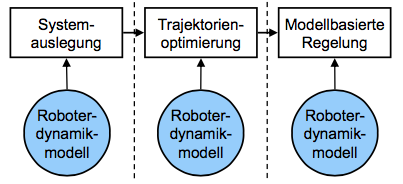
\includegraphics [scale=0.8]{dynamisch}
    \caption{Phasen von Roboter Entwicklung und -Betrieb}
\end{figure}
\begin{compactitem}
    \item Getrennte Modellierung in unterschiedlichen Phasen.
    \item Hoher Zeitaufwand, Fehler und Inkonsistenzen wahrscheinlich.
    \item Wiederverwendbarkeit des dyn. Modells schwierig bei Änderung.
\end{compactitem}

\mparagraph{Generalisierte Koordinaten}
Reduzierter Satz von Koordinaten, der den aktuellen Systemzustand vollsätndig beschreibt. Alle
Koordinaten des Satzes sind voneinander unabhängig.\\
Generalisierte Koordinaten berücksichtigen alle Zwangsbedinungen des Systems.

\mparagraph{Bewegungsgleichung}
\begin{displaymath}
     Q = M(q) \cdot \ddot{q} + n(\dot{q},q) + g(q) + R \cdot \dot{q}
\end{displaymath}
\begin{compactitem}
    \item $Q$: $n \times 1$ Vektor der Stellkräfte und -momente (Generalisierte Kräfte)
    \item $M(q)$: $n \times n$ Massenträgheitsmatrix
    \item $n(\dot{q},q)$: $n \times 1$ Vektor mit Zentrifugal- und Corioliskomponenten
    \item $g(q)$: $n \times 1$ Vektor mit Gravitationskomponenten
    \item $R$: $n \times n$ Diagonalmatrix zur Beschreibung der Reibungskräfte
    \item $q$: $n \times 1$ Winkellagen des Manipulators
\end{compactitem}

\subsection{Direktes dynamisches Problem}
Aus äußeren Kräften und Momenten sowie Anfanszustand wird die sich ergebende Bewegungsänderung
berechnet.

Gegeben: $Q(t)$, Gesucht: $q(t), \dot{q(t)}, \ddot{q(t)}$ \\
$\Rightarrow$ Gleichung auflösen nach $q(t), \dot{q(t)}, \ddot{q(t)}$
\subsection{Inverses dynamisches Problem}
Aus den gewünschten Bewegungsparametern sollen die erforderlichen Stellkräfte und Stellmomente ermittelt
werden.
Gegeben: $q(t), \dot{q(t)}, \ddot{q(t)}$, Gesucht: $Q(t)$\\
$\Rightarrow$ Gleichung auflösen.

\subsection{Lagrange Methode}
\mparagraph{Bewegungsgleichung}
\begin{align}
    Q_i &= \frac{d}{dt}(\frac{\partial L}{\partial \dot{q}_i}) - \frac{\partial L}{\partial q_i} \\
    L &= E_\text{kin} - E_\text{pot}
\end{align}
\mparagraph{Eigenschaften}
\begin{compactitem}
    \item einfaches Aufstellen der Gleichungen
    \item geschlossenes Modell
    \item analytisch auswertbar
    \item Berechnung sehr umfangreich $O(n^3)$
    \item nur Antriebsmomente werden berechnet
\end{compactitem}
\subsection{Newton-Euler Methode}
